In this section, we try to understand the behavior of \pred\ and its ability to exploit the reward correlation across tasks under a \emph{linear multivariate Gaussian model}. In this model, the hidden task parameter, $\btheta_*$, is a random variable drawn from a multi-variate Gaussian distribution \citep{bishop2006pattern} and the feedback follows a linear model.
%
We study this setting since we can estimate the Linear Minimum Mean Square Estimator (LMMSE) in this setting \citep{carlin2008bayesian, box2011bayesian}. 
%
This yields a posterior prediction for the mean of each action over all tasks on average, by leveraging the linear structure when $\btheta_*$ is drawn from a multi-variate Gaussian distribution. 
%
So we can compare the performance of \pred\ against such an LMMSE and evaluate whether it is exploiting the underlying linear structure and the reward correlation across tasks. We summarize this as follows:

\begin{tcolorbox}
\customfinding \pred\ learns the reward correlation covariance matrix from the in-context training data $\Htr$ and acts greedily on it.
\end{tcolorbox}

%
% Recall that the key insight for implementing \pred\ is that there is a common dependency across the tasks given a particular feedback structure. So as the number of tasks increases, \pred\ can learn this common reward structure and leverage it to predict the mean rewards of actions.
%
% We now show that \pred\ performs close to a Bayesian linear regression baseline that also does not have access to feature information but can evaluate the common dependency optimally.
%
% Such connections between transformers and Bayesian models have also been made in \citet{chen2021decision,muller2021transformers,lee2023supervised, yang2023bayesian}.

% \smnote{We will look into a very particular setting, where we know the optimal thing to do. So we compare this optimal predictor with that of the \pred. The dependency structure persists across tasks given the linear setting. Pure Gaussian model, where the probabilistic structure is known.}


% \smnote{Put throughout the paper that, fix a structure, linear or non-linear setting. Then there is common dependency across the tasks. \pred\ exploits this structure to better predict the rewards for an unseen task. The transformer model are good in this.}

% \smnote{prelim focuses on linear bandit setting, change it to $f(x, \btheta)$}

% \smnote{Compare it to a theoretical baseline}

% In \citet{chen2021decision,muller2021transformers,lee2023supervised, yang2023bayesian} the authors draw a connection between transformers and Bayesian models. Following this prior line of work we now show that \pred\ behaves similarly to Bayesian linear regression \citep{carlin2008bayesian, box2011bayesian}. Before we show our result we discuss the following well-known result from Bayesian linear regression.



\begin{wrapfigure}{L}{0.4\textwidth}
\centering
% \vspace*{-1.5em}
   \hspace*{-1.2em}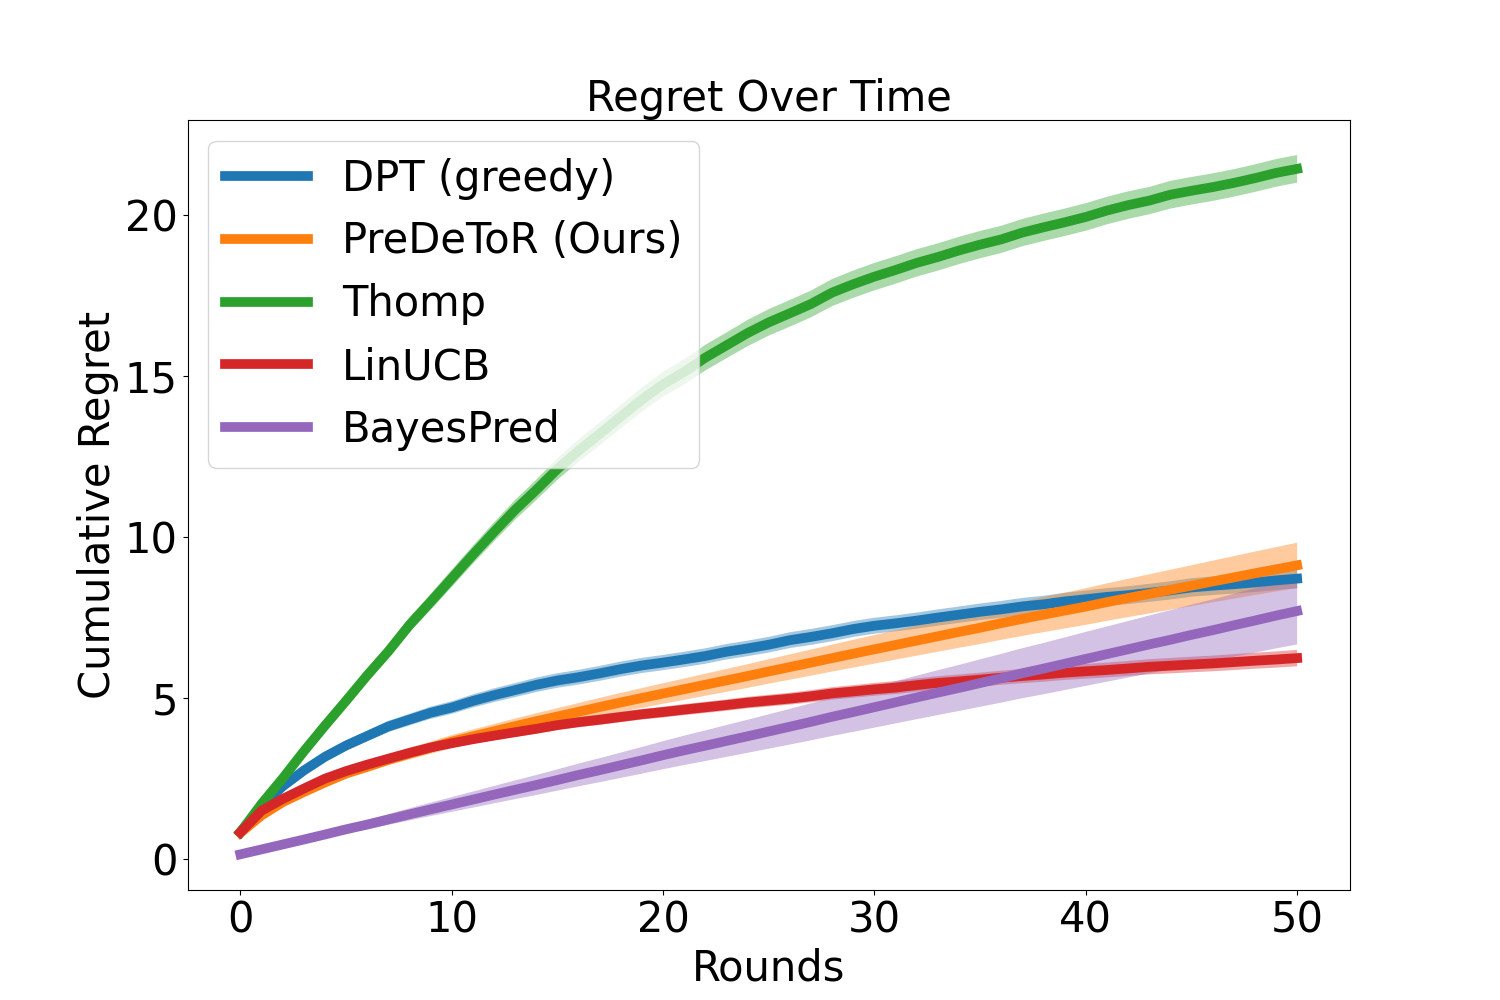
\includegraphics[scale = 0.15]{img/final/Understanding/BP_tr_lr0.00015_do0_embd32_layer4_head4_envs200000_hists1_samples1_var0.3_cov0.0_H51_d20_lind5_seed1_testcov0.0_hor51.pkl.png}
   \vspace*{-1.0em}
   %
  \caption{\label{fig:bp-tr}\bayes\ Performance}
  % \vspace*{-1.5em}
\end{wrapfigure}
%
%
% \begin{figure}[!hbt]
% \centering
% \begin{tabular}{cc}
% \subfigure[\bayes\ at train time]{\hspace*{-1.5em}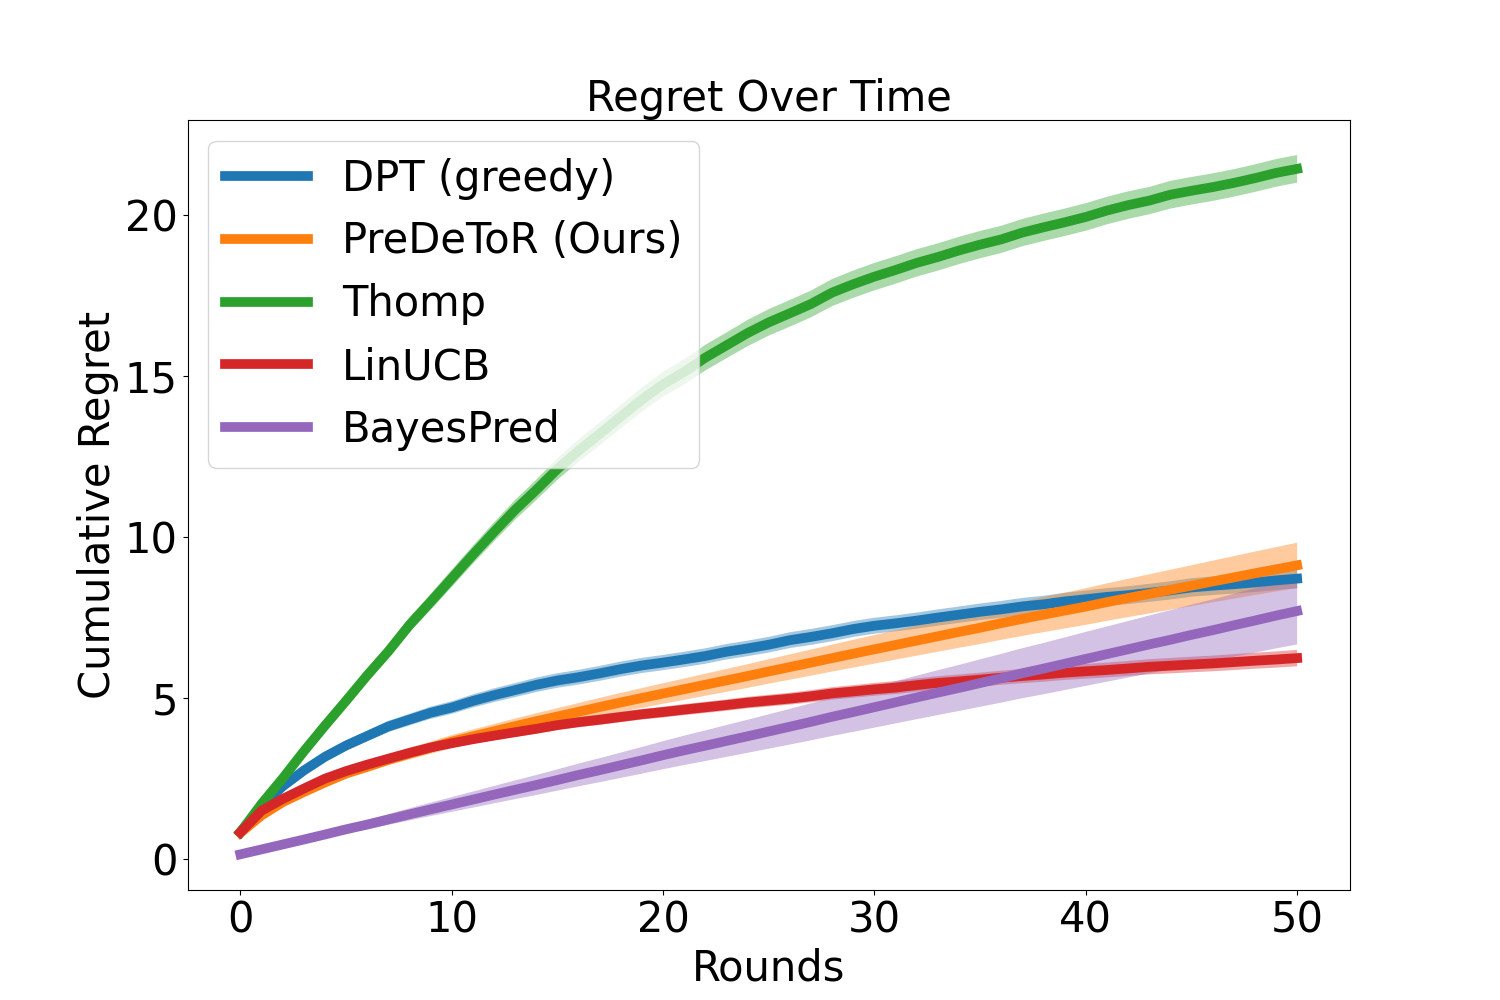
\includegraphics[scale = 0.1]{img/final/Understanding/BP_tr_lr0.00015_do0_embd32_layer4_head4_envs200000_hists1_samples1_var0.3_cov0.0_H51_d20_lind5_seed1_testcov0.0_hor51.pkl.png}\label{fig:bp-tr}} &
% %%%%%%%%%%
% \hspace*{-1.5em}\subfigure[\bayes\ at test time]{\includegraphics[scale = 0.1]{img/final/Understanding/BP_ts_lr0.00015_do0_embd32_layer4_head4_envs200000_hists1_samples1_var0.3_cov0.0_H51_d20_lind5_seed1_testcov0.0_hor51.pkl copy.png} \label{fig:bp-ts}}
% %%%%%%%%%%%%%%%%%%%%%%%
% \end{tabular}
% \vspace*{-1em}
% \caption{In the \bayes\ at train and test time, the reward covariance matrix is estimated from train data and test data respectively. The horizontal axis is the number of rounds. Confidence bars show one standard error.}
% \label{fig:expt-bayes}
% \vspace{-0.7em}
% \end{figure}

% Consider the linear feedback setting consisting of $A$ actions. Let the hidden task parameter $\btheta_{*}$ be a random variable such that $\btheta_{*}\sim\N(0,\sigma^2_{\btheta}\bI_d)$. Recall that the reward of the action $\bx_{t}$ at round $t$ is $r_{t} = \bx_{t}^\top\btheta_{*} + \eta_{t}$ where $\eta_{t}$ is the $\sigma^2$-sub-Gaussian noise. Note that we dropped the indexing by task, as $\btheta_{*}$ is a random variable now.
% %
% Let the learner collect $n$ rounds of data and observe the feature matrix $\bH_n \in \R^{n\times d}$ and reward vector $\bY_n\in \R^n$. Then the following lemma shows the prediction of the means of each of the $A$ actions.
% \begin{customlemma}{1}
% \label{lemma:bayes-reg}
%     Let $\bH_n \in \R^{n\times d}$ be the observed feature matrix and $\bY_n\in \R^n$ be the observed reward vector. Then the predicted mean vector $\wmu_m \in\R^A$ is given by
%     \begin{align*}
%         \wmu_m = \sigma^2_{\btheta}\bX_m\bH_n^\top\left(\sigma^2_{\btheta}\bH_n\bH_n^\top + \sigma^2\bI_{n\times n}\right)^{-1}\bY_n
%     \end{align*}
% \end{customlemma}
% The proof of this above lemma is given in \Cref{app:proof-lemma-1} and follows by using a standard linear regression argument by constructing the posterior estimate of $\btheta_{*}$. However, note that in our setting the learner is a weak demonstrator $\pi^w$ and hence does not have access to feature space $\X$. This motivates us to study a new Bayesian linear predictor that can inform us of the lower bound to the cumulative regret achieved by \pred.
%
%
Consider the linear feedback setting consisting of $A$ actions and the hidden task parameter $\btheta_{*}\sim\N(0,\sigma^2_{\btheta}\bI_d)$. The reward of the action $\bx_{t}$ at round $t$ is given by $r_{t} = \bx_{t}^\top\btheta_{*} + \eta_{t}$, where $\eta_t$ is $\sigma^2$ sub-Gaussian.
%
Let $\pi^w$ collect $n$ rounds of pretraining in-context data and observe $\{I_t, r_t\}_{t=1}^n$. Let $N_n(a)$ denote the total number of times the action $a$ is sampled for $n$ rounds. Note that we drop the task index $m$ in these notations as the random variable $\btheta_{*}$ corresponds to the task.
%
%
Define the matrix $\bH_n \in \R^{n \times A}$ where the $t$-th row represents the action $I_t$ for $t\in [n]$. 
%
The $t$-th row of $\bH_n$ is a one-hot vector with the  $I_t$-th component being 1. We represent each action by one hot vector because we assume that this LMMSE does not have access to the feature vectors of the actions similar to the \pred~for fair comparison.
%
Then define the reward vector $\bY_n \in \R^n$ where the $t$-th component is the reward $r_t$ observed for the action $I_t$ for $t\in[n]$ in the pretraining data.
% after $n$ rounds of observed rewards.
%
Define the diagonal matrix $\bD_A\in\R^{A\times A}$ estimated from pretraining data as follows
\begin{align}
    \bD_A(i,i) &= \begin{cases}
        \frac{\sigma^2}{N_n(a)}, \text{ if } N_n(a) > 0\\ \label{eq:D-matrix}
        %%%%%%%%%%%%
        = 0, \text{ if } N_n(a) = 0
    \end{cases}
    \vspace*{-1em}
\end{align}
%
where the reward noise being $\sigma^2$ sub-Gaussian is known. 
%
Finally define the estimated reward covariance matrix $\bS_A\in\R^{A\times A}$ as $\bS_A(a,a') = \wmu_n(a)\wmu_n(a')$, where $\wmu_n(a)$ is the empirical mean of action $a$ estimated from the pretraining data. This matrix captures the reward correlation between the pairs of actions $a,a'\in [A]$.
%
%
% Let $N_t(a)$ denote the number of times each action $a$ is sampled. Let the observed reward vector be $\bY_n\in \R^n$.
%
% Then the following lemma shows the posterior prediction of the means of each of the $A$ actions by the learner using a linear feedback model.
%
% Let $\wmu_m \in\R^A$ be the optimal posterior prediction of the mean reward vector. 
%
Then the posterior average mean estimator $\wmu\in\R^A$ over all tasks is given by the following lemma. The proof is given in \Cref{app:proof-lemma-2}.
\begin{customlemma}{1}
\label{lemma:bayes-reg-1}
    Let $\bH_n$ be the action matrix, $\bY_n$ be the reward vector and $\bS_A$ be the estimated reward covariance matrix. Then the posterior prediction of the average mean reward vector $\wmu$ over all tasks is given by
    \begin{align}
        \wmu = \sigma^2_{\btheta}\bS_A\bH_n^\top\left(\sigma^2_{\btheta}\bH_n(\bS_A + \bD_A)\bH_n^\top\right)^{-1}\bY_{n}. \label{eq:mu}
    \end{align}
\end{customlemma}
%
The $\wmu$ in \eqref{eq:mu} represents the posterior mean vector averaged on all tasks. So if some action $a\in [A]$ consistently yields high rewards in the pretraining data then $\wmu(a)$ has high value. Since the test distribution is the same as pretraining, this action on average will yield a high reward during test time.  
% and follows a similar analysis as in \Cref{lemma:bayes-reg}. 
% Note that the reward correlation covariance matrix $\bS_A$ can be estimated from the pretraining data.
%
% Once the average posterior mean vector $\wmu\in\R^A$ is estimated, the learner chooses the action $I_{t} =\argmax_a \wmu(a)$, at round $t$. 
%

We hypothesize that the \pred\ is learning the reward correlation covariance matrix from the training data $\Htr$ and acting greedily on it. To test this hypothesis, we consider the greedy \bayes\ algorithm that first estimates $\bS_A$ from the pretraining data. It then uses the LMMSE estimator in \Cref{lemma:bayes-reg-1} to calculate the posterior mean vector $\wmu$, and then selects $I_{t} =\argmax_a \wmu(a)$ at each round $t$. Note that \bayes\ is a greedy algorithm that always selects the most rewarding action (exploitation) without any exploration of sub-optimal actions. 
%
Also the \bayes\ is an LMMSE estimator that leverages the linear reward structure and estimates the reward covariance matrix, and therefore can be interpreted as a lower bound to the regret of \pred.
%
The hypothesis that \bayes\ is a lower bound to \pred\ is supported by \Cref{fig:bp-tr}.  In \Cref{fig:bp-tr} the reward covariance matrix for \bayes\ is estimated from the $\Htr$ by first running the \ts\ ($\pi^w$). Observe that the \bayes\ has a lower cumulative regret than \pred\ and almost matches the regret of \pred\ towards the end of the horizon. 
%
Also note that \linucb\ has lower cumulative regret towards the end of horizon as it leverages the linear structure and the feature of the actions in selecting the next action.
%
% Similarly for test time \bayes\ in \Cref{fig:bp-ts} the reward covariance matrix is estimated from the $\Dts$ using the data collected by \ts. 
%
% This supports our hypothesis that \pred\ is inherently doing a Bayesian linear regression on the linear feedback setting from the data collected by $\pi^w$ even though it does not have access to the feature space.


% Finally we finish this section by showing that \pred\ (similar to \dpt) is equivalent to posterior sampling. 
%
%
%
% This means that the trajectories generated by a pretrained $\T_\bw$ will follow the same distribution as those from a well-specified PS algorithm. In particular, let PS use the well-specified prior $\cTp$. Let $m$ be an arbitrary task. Let
% %
% $P_{p s}\left(\cdot \mid \H, m\right)$ and $P_{\T_\bw}\left(\cdot \mid \H, m\right)$ denote the distributions over trajectories $\xi_n \in(\mathcal{A})^n$ generated from running PS and $\T_\bw(\cdot \mid \cdot, \H, \cdot)$, respectively, in task $m$ given historical data $\H$.

% \begin{theorem}
    
% \end{theorem}
% Theorem 1 (DPT $\Longleftrightarrow$ PS). Let the above assumptions hold. Then, $P_{p s}\left(\xi_H \mid D, \tau_c\right)=$ $P_{M_\theta}\left(\xi_H \mid D, \tau_c\right)$ for all trajectories $\xi_H$.